\section{Czytania}

\begin{itemize}
      \item wszyscy procesyjnie udają się do ołtarza dłuższą drogą, nie niesie
            się żadnych przedmiotów, nie wykonuje się skłonu
      \item \ii~ ubrany w albę, czarną stułę i biret
      \item po dojściu do ołtarza ministranci rozchodzą się na swoje miejsca w
            chórze, \aa1\aa2~ do krednecji (patrz Rys. \ref{fig:lezenie})
      \item \cc1 odbiera od \ii~ biret, odnosi go na sedillę, a z kredencji
            przynosi księgę OHS

            \begin{figure}[h]
                  \centering
                  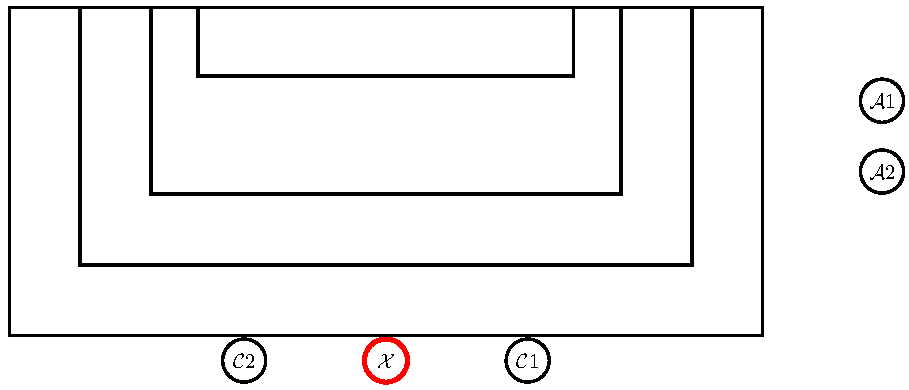
\includegraphics[scale=0.7]{Piatek/Wejscie.pdf}
                  \caption{Leżeniem krzyżem (prostracja)}
                  \label{fig:lezenie}
            \end{figure}

      \item \ii~ pada na twarz, ministranci klękają na posadzce i kłaniają się
            głęboko
      \item \ii~ wraz z \cc1 i \cc2 wstają, ministranci prostują się, śpiewana
            jest modlitwa przy stopniach ołtarza
      \item po modlitwie wszyscy powstają, robią skłon i udają się na swoje
            miejsca (\ii, \aa1, \aa2 i \cc1 -- na sedile)
      \item ministranci w chórze siadają w tym samym momencie, co \aa\aa
      \item \cc2 zabiera poduszkę ze stopni ołtarza
      \item \tt1 przynosi pulpit po stronie epistoły
      \item \bb~ przynosi księgę OHS i stając przed \ii~ siedzącym na sedilii,
            otwiera lekcję, a \cc1 wskazuje właściwy tekst
      \item wyznaczony ministrant śpiewa pierwszą lekcję
      \item po lekcji śpiewane jest responsorium
      \item następnie \ii~ odmawia modlitwę – na \textit{Oremus} wszyscy wstają,
            na \textit{Flectamus genua} klękają, na \textit{Levate} wstają, po
            skończonej modlitwie siadają
      \item śpiewana jest kolejna lekcja i responsorium
      \item w czasie śpiewu drugiego rosponsorium \cc2 przenosi pulpit przed
            \ii, a \cc1 ustawia na nim OHS odebrany od \bb
      \item \ii~ wstaje i pochylony odmawia modlitwę przed Ewangelią, po czym
            rozpoczyna ciche czytanie Pasji. Towarzyszy mu \cc1, przewracając
            kartki. Po przeczytaniu przez \ii~ Pasji, \cc2 zabiera pulpit wraz z OHS
      \item chór wstaje dopiero kiedy śpiewacy rozpoczną Pasję. Chór nie
            wykonuje rewerencji z \ii, nie przyklęka z \ii, nie zwraca się w
            żadną stronę
      \item po zaśpiewaniu słów oddał ducha wszyscy klękają i przez chwilę modlą
            się w ciszy
      \item po zakończeniu \textbf{nie} odpowiada się \textit{Laus Tibi, Christe}
\end{itemize}